\documentclass[tikz,border=3mm]{standalone}
\usetikzlibrary{arrows.meta,decorations.markings}

\begin{document}
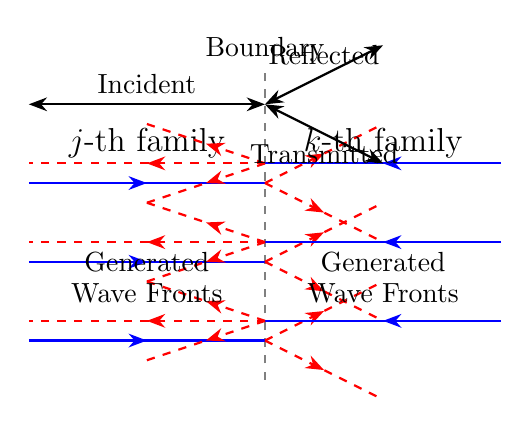
\begin{tikzpicture}[>=Stealth,
    wave/.style={thick, blue, decoration={markings, mark=at position 0.5 with {\arrow{>}}}, postaction={decorate}},
    reflected/.style={thick, dashed, red, decoration={markings, mark=at position 0.5 with {\arrow{>}}}, postaction={decorate}},
    boundary/.style={thick, dashed, gray}
]
    % Boundary line
    \draw[boundary] (3,0) -- (3,4);
    
    % Left side (j-th family)
    \foreach \y in {0.5,1.5,2.5} {
        \draw[wave] (0,\y) -- (3,\y);
        \draw[reflected] (3,\y) -- (4.5,\y + 0.75);
        \draw[reflected] (3,\y) -- (4.5,\y - 0.75);
    }
    \node at (1.5,3) {\large $j$-th family};
    
    % Right side (k-th family)
    \foreach \y in {0.75,1.75,2.75} {
        \draw[wave] (6,\y) -- (3,\y);
        \draw[reflected] (3,\y) -- (1.5,\y + 0.5);
        \draw[reflected] (3,\y) -- (1.5,\y - 0.5);
        \draw[reflected] (3,\y) -- (0,\y);
    }
    \node at (4.5,3) {\large $k$-th family};
    
    % Labels
    \node at (3,4.2) {Boundary};
    \node at (1.5,1.5) {Generated};
    \node at (1.5,1.1) {Wave Fronts};
    \node at (4.5,1.5) {Generated};
    \node at (4.5,1.1) {Wave Fronts};
    
    % Annotations
    \draw[thick, <->] (0,3.5) -- (3,3.5) node[midway,above] {Incident};
    \draw[thick, <->] (3,3.5) -- (4.5,4.25) node[midway,above] {Reflected};
    \draw[thick, <->] (3,3.5) -- (4.5,2.75) node[midway,below] {Transmitted};
\end{tikzpicture}
\end{document}